\chapter{Implementazione}
Successivamente alla definizione dei requisiti funzionali e non funzionali dell'applicazione e alla descrizione dei diversi casi d'uso che coinvologono l'utente e altri sistemi esterni, si passa all'implementazione vera e propria dell'applicativo.
\section{Struttura iniziale di un'Applicazione in React Native}
Come strumento per lo sviluppo dell'applicazione \`e stato usato Expo, il quale permette di creare un nuovo progetto tramite l'utilizzo di questo comando all'interno del proprio terminale:
\begin{itemize}
    \item npx create-expo-app my-app
\end{itemize}
Quando si vuole sviluppare un'applicazione in React Native \`e richiesto di seguire una ``gerarchia delle cartelle" gestita da Expo. Quando si utilizza il comando sopra indicato per la creazione di un nuovo progetto,
queste sono le cartelle e i file che vengono creati:
\begin{itemize}
    \item La cartella ``node modules" contiene tutte le dipendenze e i package necessari al funzionamento dell'applicazione. Ogni volta che viene installato un nuovo package realizzato da terze parti, lo si ritrova in tale cartella.
    \item Il file ``package.json" permette di tenere traccia delle varie dipendenze, indicando quale versione di ogni package deve essere scaricata.
    \item Il file ``App.js" contiene il primo componente che viene mostrato ogni volta che viene aperta l'applicazione.
    \item La cartella ``assets" contiene le immagini che verranno utilizzate all'interno dell'applicazione.
\end{itemize}
\begin{figure}[h]
    \centering
    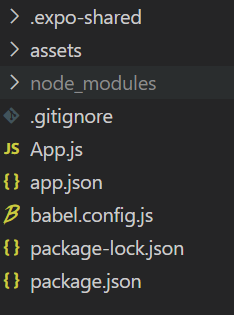
\includegraphics[width=5cm, height=7cm]{images/ExpoFileCartelle.png}
    \caption[differenzeiteot]{}
    \label{fig:ExpoCartelleFile}
\end{figure}
\section{Navigazione all'interno dell'Applicazione}
Ogni applicazione \`e composta da diversi screen ed \`e necessario permettere all'utente di transitare tra di essi. Per svolgere questa operazione \`e stata usata la 
libreria \textit{React Navigation}, la quale fornisce diversi componenti e funzioni per la gestione della navigazione all'interno dell'app. In particolare all'interno 
dell'applicativo ho utilizzati \cite{ReactNavigationContainer}\cite{ReactNavigationStackNavigator}:
\begin{itemize}
    \item NavigationContainer: \`e un componente responsabile della gestione dello stato dell'applicazione, del collegamento del top-level navigator all'ambiente dell'applicazione e dell'integrazione con la piattaforma specifica su cui verr\`a installata.
          Solitamente viene utilizzato una sola volta all'interno dell'applicativo e viene inserito nel file App.js/App.tsx. Lo scopo principale di questo componente \`e la gestione della navigazione tra i vari navigator che verranno inseriti all'interno dell'applicazione. Per poterlo utilizzare \`e necessario importarlo dalla libreria \textit{react-navigation}.
    \item Stack Navigator: fornisce all'applicazione la possibilit\`a di transitare attraverso gli screen e gestire la storia della navigazione. Ogni volta che l'utente transita da uno screeen ad un altro viene fatta un'operazione di ``push" e fa s\`i che il nuovo screen venga messo in cima allo stack. Invece, ogni volta che l'utente vuole tornare
          alla schermata precedente, viene fatta un'operazione di ``pop" e lo screen in cima allo stack viene rimosso. Per poterlo utilizzare \`e necessario importare la funzione ``createStackNavigator", la quale restituisce un oggetto che contiene due propriet\`a: \textit{Screen} e \textit{Navigator}.
          Entrambi sono dei ``React component" che vengono utilizzati per configurare il navigator. Il \textit{Navigator} permette di definire la route iniziale, ossia lo screen da mostrare per primo ogni volta che viene invocato lo Stack Navigator; questo componente dovr\`a contenere i vari \textit{Screen} i quali consentono di definire i vari schermi verso cui l'utente pu\`o transitare.
          Lo \textit{Screen} presenta 3 prop:
          \begin{list}{*}{}
              \item Name: il nome della route.
              \item Component: il JSX component da mostrare.
              \item Option: un oggetto che definisce alcune propriet\`a con cui lo schermo dovr\`a essere presentato.
          \end{list}
\end{itemize}
Tramite l'utilizzo della libreria {}(\textit{React Navigation}) \`e possibile annidare pi\`u navigator in modo da definire una gerarchia. L'importante \`e che in cima ad essa si abbia il NavigationContainer.\\
\begin{figure}[h]
    \centering
    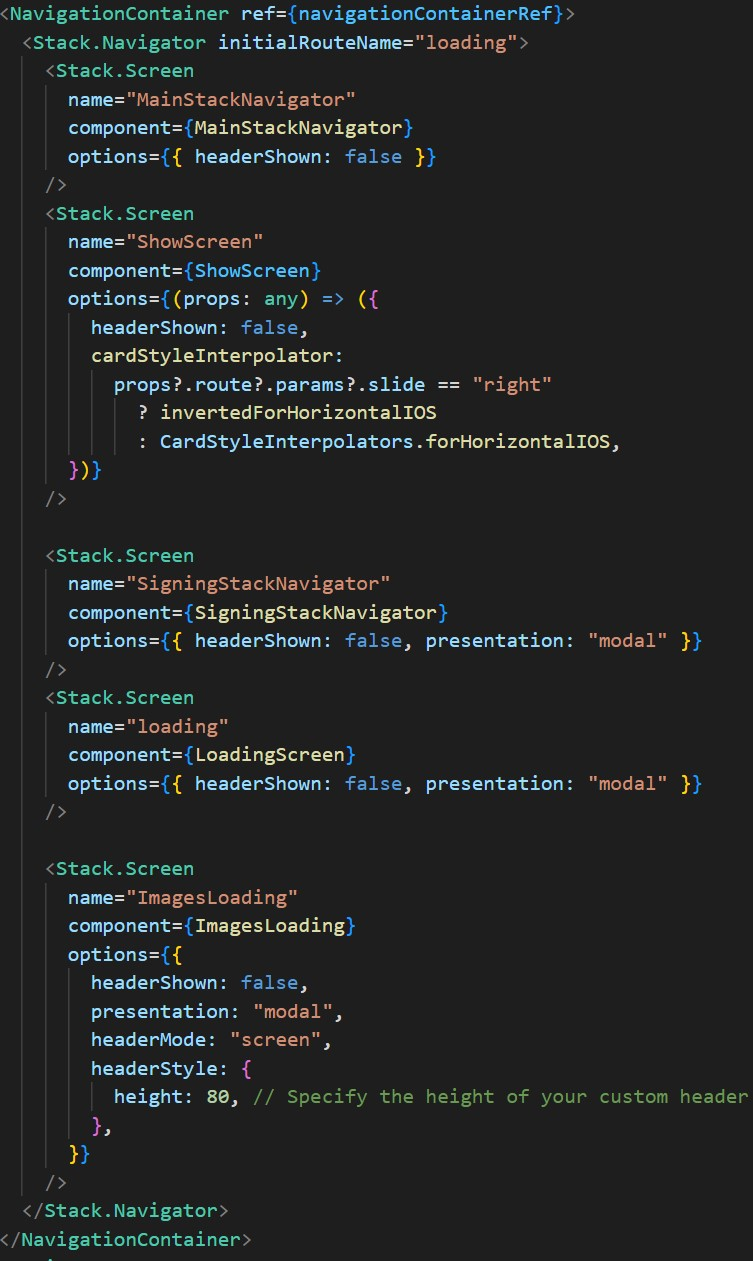
\includegraphics[width=9cm, height=15cm]{images/navigationCode.jpg}
    \caption[differenzeiteot]{Frammento di codice che gestisce la navigazione tra gli schermi}
    \label{fig:Navigation code}
\end{figure}

nella figura 3.2, viene mostrato un frammento di codice \`e stato preso dal file App.tsx . Come si pu\`o vedere il NavigationContainer \`e il componente in cima alla gerarchia e va ad avvolgere i vari Stack Navigator:
\begin{enumerate}
    \item Il primo \`e quello immediatamente successivo al NavigationContainer e viene utilizzato per gestire la transizione verso:
          \begin{list}{*}{}
              \item Gli altri due Stack Navigator
              \item Lo schermo di loading iniziale
              \item Lo schermo per la visualizzazione delle immagini memorizzate in cache
              \item Lo screen che mostra i dettagli di un'immagine
          \end{list}
    \item Il Secondo si chiama MainStackNavigator e gestisce la navigazione tra l'index Screen e il Seach Screen.
    \item Il terzo si chiama SigningStackNavigator e gestisce la navigazione tra lo screen di sign in e quello di sign up.
\end{enumerate}

\section{Stati all'Interno dell'Applicazione}
All'interno dell'applicazione vi sono diversi stati che vengono continuamente aggiornati; per tenere traccia di ognuno di essi sono stati utlizzati le librerie \textit{redux} e \textit{react-redux}.
Attraverso di esse si va a creare uno \textit{store} che contiene l'intero stato dell'applicazione come un semplice oggetto JavaScript. 

Per poter modificare gli stati vengono utilizzate delle funzioni pure chiamate
\textit{reducers} che specificano come cambia lo stato in risposta ad una \textit{action}. I \textit{reducers} prendono come argomento un'azione con un payload e restituiscono un nuovo stato basato sull'azione passata. Essendo funzioni pure non modificano i dati
dell'oggetto che viene passato e non eseguono alcun effetto collaterale nell'applicazione; dato lo stesso stesso oggetto dovrebbero produrre sempre lo stesso risultato.
Le \textit{action} devono avere una propriet\`a ``type" per indicare il tipo di azione da eseguire. Esse rappresentano l'unica fonte di informazioni per lo \textit{store}\cite{ReduxSite}.
%Le \textit{action} passate ad ogni reducer sono degli oggetti JavaScript inviati attraverso il metodo nativo di React, chiamato dispatch(). 

\begin{figure}[h]
    \begin{minipage}[b]{0.47\textwidth}
        \centering
        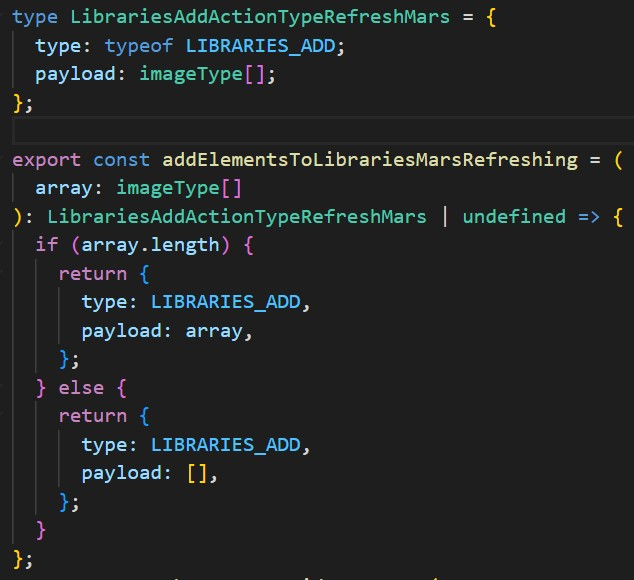
\includegraphics[width=6cm, height=6cm]{images/ActionRedux.jpg}
        \caption{\label{f_etichetta1} Esempio di \textit{action}}
    \end{minipage}
    \hfill
    \begin{minipage}[b]{0.47\textwidth}
        \centering
        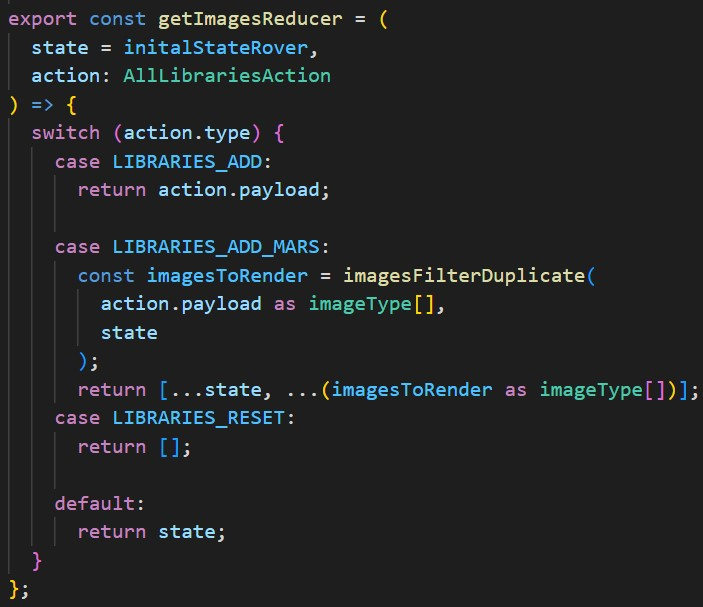
\includegraphics[width=6cm, height=6cm]{images/ReduxReducersFunction.jpg}
        \caption{\label{f_etichetta2}Esempio di \textit{reducer}}
    \end{minipage}
\end{figure}

Sia le \textit{action} che i \textit{reducer} vengono definiti come delle arrow function. La \textit{action} rappresentata nella fig 3.3 viene utilizzata per indicare che l'array contenente le immagini che devono essere visualizzate a schermo, deve essere aggiornato.
Un \textit{action} ritorna sempre un oggetto che contiene due propriet\`a ovvero type e payload: La prima viene utilizzata per indicare al \textit{reducer} quale azione deve essere eseguita, mentre la seconda rappresenta il contenuto con cui deve essere aggiornato lo stato all'interno dello store.

Il \textit{reducer} rappresentato nella fig 3.4, riceve sempre due parametri, che sono state e action: il primo rappresenta lo stato memorizzato nello store e viene sempre passato da quest'ultimo ogni volta che il \textit{reducer} viene invocato; l'\textit{action} rappresenta l'azione che il \textit{reducer} deve eseguire.
In base all'azione passata si entrer in uno dei diversi ``case" dello switch.

Supponendo che venga eseguita l'\textit{action} mostrata nella fig 3.3, si entrerebbe nel primo ``case" dello switch e si andrebbe a sostituire lo stato attuale con il payload fornito dall'\textit{action}.

Le \textit{action} passate ad ogni reducer sono degli oggetti JavaScript inviati attraverso il metodo nativo di React, chiamato dispatch() che prende come parametro la \textit{action} stessa. Per poter invocare questo metodo 
\`e necessario utilizzare un hook, chiamato ``useDispatch".

Oltre a poter memorizzare gli stati all'interno dello store \`e anche possibile accedere ai dati contenuti in essi attraverso un altro hook, chiamato ``useSelector".
Gli state memorizzati nello store sono:
\begin{enumerate}
    \item dataRover: un oggetto JavaScript che contiene le informazioni riguardanti la ricerca fatta dall'utente.
    \item images: un array che contiene tutte le immagini che, una volta filtrate, devono essere visualizzate a schermo.
    \item imagesHide: un array che contiene tutte le immagini che sono state occultate dall'utente.
    \item loading: \`e una variabile booleana che indica quando deve essere presentata all'utente un'animazione.
    \item search: \`e una variabile booleana che permette di avviare una procedura di ricerca.
    \item sign: viene utilizzato per memorizzare il JWT che \`e stato fornito all'utente in fase di registrazione o login.
\end{enumerate}
\begin{figure}[h]
    \centering
    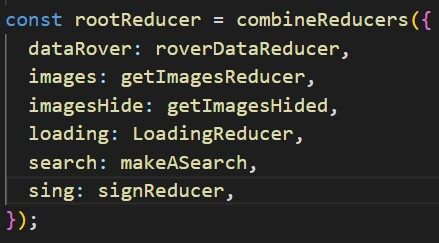
\includegraphics[width=9cm, height=5cm]{images/state.jpg}
    \caption[differenzeiteot]{A sinistra lo state memorizzato nello store e a destra il rispettivo reducer}
    \label{fig:state}
\end{figure}
\section{Fetching delle Immagini}
Ogni volta che l'utente effettua una nuova ricerca digitando il nome di un Rover oppure la data solare in cui sono state scattate le immagini, viene effettuata una richiesta HTTP ai server della Nasa; in particolare, viene effettuata una GET request \cite{Axios}.

Per effettuare richieste HTTP \`e stato utilizzato Axios, un Client HTTP che ritorna una \textit{Promise}, la quale rappresenta l'eventuale completamento {}(o fallimento) di un'operazione asincrona e il suo conseguente valore \cite{Promise}.
\begin{figure}[h]
    \centering\`a
    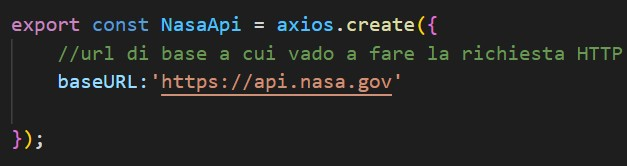
\includegraphics[width=6cm, height=2cm]{images/baseUrl.jpg}
    \caption[differenzeiteot]{Base URL}
    \label{fig:baseUrl}
\end{figure}
\begin{figure}[h]
    \centering
    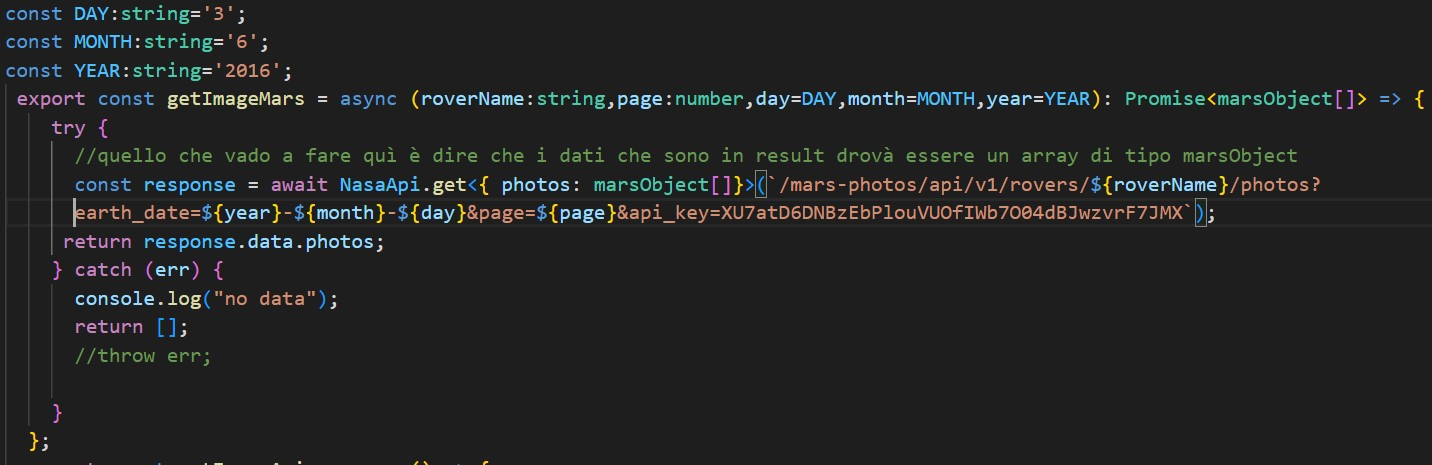
\includegraphics[width=14cm, height=5cm]{images/getRequest.jpg}
    \caption[differenzeiteot]{Esempio di richiesta GET}
    \label{fig:getRequest}
\end{figure}

Per poter eseguire una GET request finalizzata al recupero delle immagini, come nella fig 3.7, \`e necessario fornire al metodo ``get" dell'Axios instance {}(creata nella fig 3.6) L'URL a cui deve deve essere effettuata la richiesta e i parametri per ricercare le immagini; in particolare questi ultimi sono:
\begin{list}{*}{}
    \item Il nome del Rover {}(required)
    \item La data solare in cui sono state scattate le foto {}(required)
    \item Il numero di pagina a cui si vuole accedere {}(optional)
\end{list}
Si evidenzia che la data solare viene impostata ad un valore iniziale in modo da poter presentare all'utente un certo tipo di immagini nel momento in cui apre l'applicazione per la prima volta.

Il metodo GET utilizzato ritorna una ``Axios Response", la quale \`e un oggetto che contiene diverse propriet\`a tra cui ``data". Attraverso essa \`e possibile accedere alla risposta fornita dai server della Nasa in formato JSON.

\section{Presentazione delle Immagini}
Per visualizzare le immagini che sono state recuperate dai server della Nasa, viene utilizzato un Core Component chiamato FlatList, reso disponibile da React Native.
Questo componente presenta diverse \textit{prop}, in particolare nel mio Applicativo sono state usate le seguenti \cite{FlatList}:
\begin{itemize}
    \item data: a questa \textit{prop} deve sempre essere passata un array; in questo caso l'array di immagini che devono essere visualizzate a schermo.
    \item renderItem: a questa \textit{prop} deve essere passata una funzione o un function component che verr\`a eseguito per ogni elemento dell'array che \`e stato fornito alla prop data.
          Nel caso di questa applicazione a renderItem viene passato un ``Function Component" chiamato \textit{PhotoComponent} il quale permette di visualizzare ognin immagine e il suo id.
    \item keyExtractor: questa \textit{prop} viene utilizzata per estrarre una chiave univoca per ogni elemento della lista. In questo modo \`e possibile riodinare gli elementi se alcuni di essi venissero
          eliminati o ne venissero aggiunti altri. In questo applicativo ad ogni elemento della lista viene associato come chiave univoca l'id di ogni immagine.
    \item listFooterComponent: questa \textit{prop} permette di visualizzare un React Element/Component alla fine della lista; in questo applcativo le viene passato un React Element chiamato \textit{FooterComponent} che permette di visualizzare due link: Privacy and Policy e Log Out.
    \item onEndReached: a questa \textit{prop} viene passata una funzione invocata ogni volta che viene raggiunta la fine della lista.
          In questo applicativo, una volta raggiunta l'ultima immagine recuperata dalla ricerca precedente, viene effettuata una nuova richiesta ai server della Nasa, utilizzando gli stessi parametri di ricerca, recuperando la pagina di immagini successiva. Quest'ultima potrebbe o meno contenere delle immagini: nel caso
          in cui ve ne siano, verranno inserite in coda all'array visualizzate a schermo; in caso contrario le immagini visibili all'utente rimarranno le stesse.
\end{itemize}

\begin{figure}[h]
    \centering
    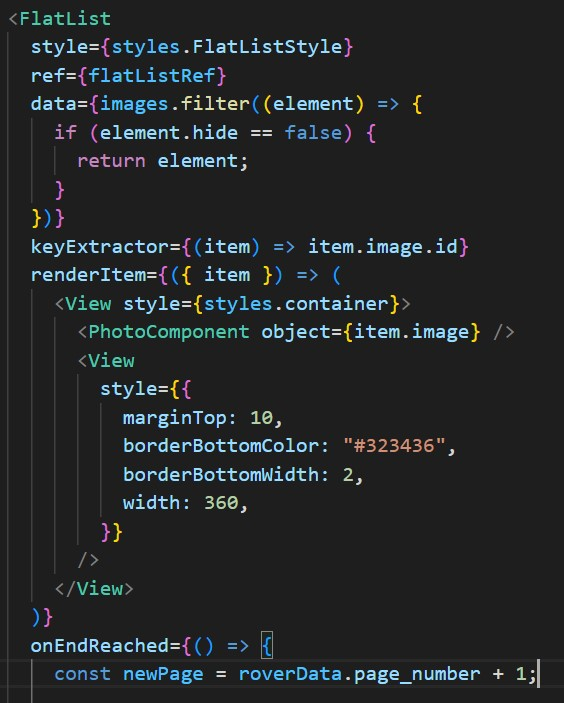
\includegraphics[width=7cm, height=10cm]{images/FlatListPrimaParte.jpg}
    \label{fig:FlatListPrimaParte}
\end{figure}

\begin{figure}[h]
    \centering
    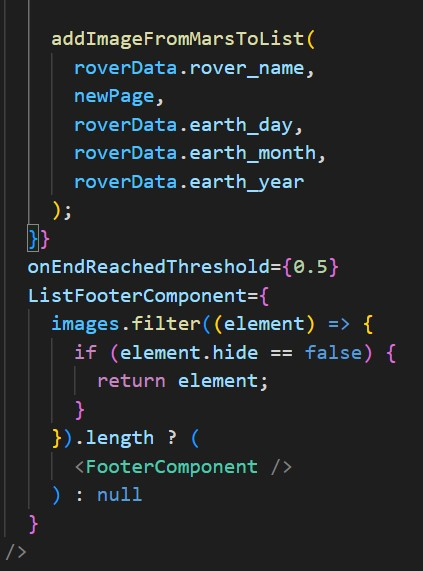
\includegraphics[width=7cm, height=10cm]{images/FlatListSecondaParte.jpg}
    \caption[differenzeiteot]{Esempio di uso della Flat List}
    \label{fig:FlatListSecondaParte}
\end{figure}

Ogni volta che l'utente chiude l'applicazione e poi la riapre, gli vengono subito mostrate delle immagini secondo dei parametri di ricerca predefiniti. Per andare a recuperare queste immagini
viene utilizzato un hook di React chiamato useEffect, al quale vengono assegnate due dipendenze: Search e allButtonColor. La prima dipendenza \`e uno state
che viene aggiornato ogni volta che un utente vuole effettuare una nuova ricerca di immagini; il secondo \`e uno state che viene aggiornato ogni volta che l'utente preme sul
pulsante ``all", esprimendo in questo modo l'intenzione di voler eseguire una ricerca.

Lo useEffect mostato nella fig 3.9 non viene eseguito solo quando l'utente apre l'applicazione per la prima volta, ma anche ogni volta che effettua una nuova ricerca di immagini.
Tutte le volte che viene eseguito il frammento di codice nella fig 3.9 viene aggiornato lo state \textit{dataRover}, andando a modificare il numero di pagina da recuperare. Inoltre viene invocata una funzione chiamata ReplaceImageFromMarsList{}(),
la quale va a recuperare le nuove immagini da mostrare all'utente.
\begin{figure}[h]
    \centering
    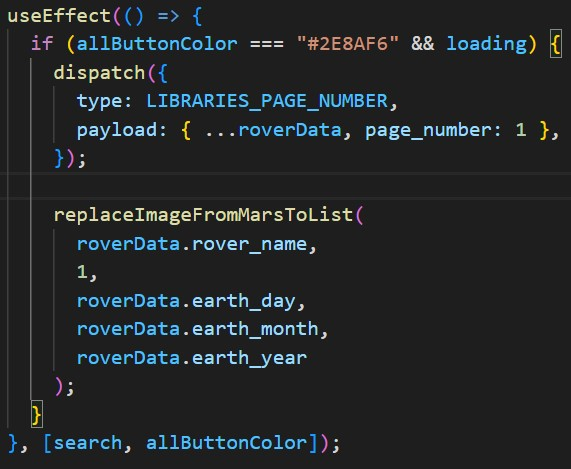
\includegraphics[width=7cm, height=7cm]{images/useEffect.jpg}
    \caption[differenzeiteot]{UseEffect per il caricamento delle immagini}
    \label{fig:useEffect}
\end{figure}
\subsection*{ReplaceImageFromMarsList()}
Come si pu\`o vedere nella fig 3.10, questa funzione richiede che le vengono passati alcuni parametri:
\begin{itemize}
    \item Il nome del Rover per cui deve essere eseguita la ricerca.
    \item La pagina che contentiene le immagini da recuperare: questa funzione viene eseguita ogni volta che l'utente vuole ricercare nuove immagini, quindi sar\`a necessario recuperare sempre la prima pagina.
    \item Gli ultimi tre parametri corrispondono al giorno, mese e anno terrestre in cui sono state scattate le foto.
\end{itemize}

Questa funzione va ad invocare un metodo, chiamato getImageMars(), il quale va ad eseguire una GET request per recuperare le nuove immagini; una volta ottenute, si controlla che l'utente abbia premuto il tasto ``Photos" e quindi voglia visualizzare o meno le immagini nascoste.
Nel primo caso si va ad aggiornare lo state ``images" con tutte le foto recuperate; nel secondo caso viene aggiornato lo state "images" solo con le immagini che l'utente non ha occultato in precedenza.

Potrebbe accadere che l'utente fornisca dei parametri di ricerca errati e in tal caso verr\`a mostrato un messaggio di errore.

Le immagini recuperate vengono mostrate a schermo solo dopo che lo state ``loading" verr\`a posto a ``false": questo avviene dopo quattro secondi tramite l'utilizzo di una funzione asincrona, chiamata setTimeout.
\begin{figure}[h]
    \centering
    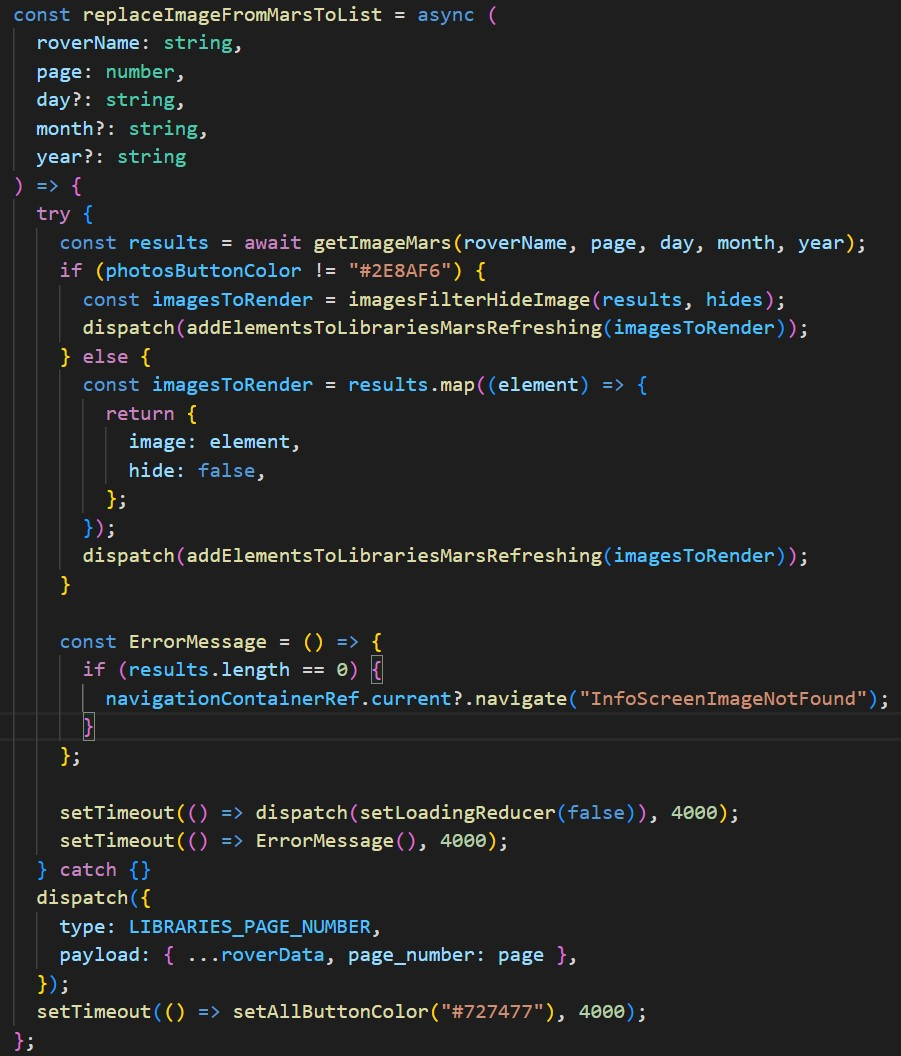
\includegraphics[width=10cm, height=14cm]{images/ReplaceImageFunction.jpg}
    \caption[differenzeiteot]{Funzione replaceImageFromMarsList}
    \label{fig:replaceImageFunction}
\end{figure}

\section{Ricerca Immagini per Nome Rover e per Data Solare}
Per poter ricercare delle immagini tramite il nome del Rover, viene fornita una search-bar il cui componente corrsipendente \`e mostrato nella fi 3.11. Quando l'utente abilita la ricerca premendo sul pulsante ``All" e poi digita nella Search-bar il nome di uno dei Rover, vengono emesse tre azioni:
\begin{itemize}
    \item Viene modificato lo state che mantiene le informazioni sui parametri di ricerca forniti dall'utente, aggiornando quindi il campo RoverName.
    \item Viene posto a true lo state ``loading", in modo da mostrare un'animazione che informi l'utente dell'avvio della ricerca.
    \item Viene modificato lo state ``search", in modo che venga eseguito lo useEffect mostrato in fig 3.9.
\end{itemize}
\begin{figure}[h]
    \centering
    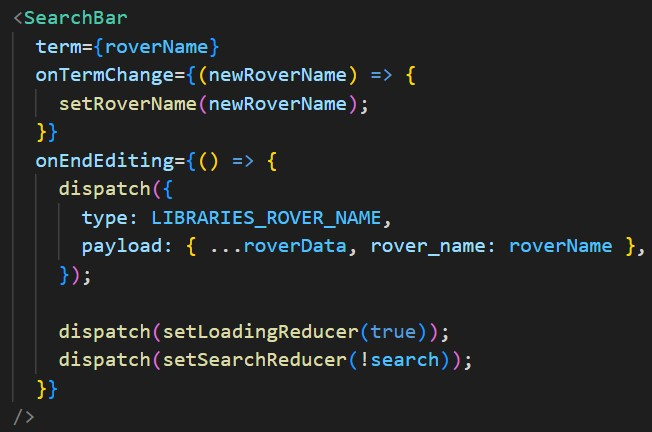
\includegraphics[width=8cm, height=6cm]{images/SearchBar.jpg}
    \caption[differenzeiteot]{Search-bar}
    \label{fig:Search-bar}
\end{figure}

Per poter ricercare delle immagini in base alla data solare vengono forniti all'utente tre campi ``input text", nei quali deve inserire giorno, mese e anno in cui sono state scattate.
Quando viene premuto il tasto ``Search by date" avviene un aggiornamento degli stati simile a quello della fig 3.11. L'unica differenza riguarda l'aggiornamento dello stato ``dataRover": invece di 
modificare il campo roverName vengono aggiornati i campi earth-day, earth-month, earth-year.

\section{Immagini Persistenti}
L'applicazione oltre a recuperare delle immagini in base ai parametri di ricerca inseriti dall'utente, deve far s\`i che vengano visualizzate solo le foto che non occultate in precedenza. Inoltre, le ultime immagini visualizzate dall'utente, devono essere presentate a quest'ultimo quando andr\`a a riaprire l'applicazione.
Per soddisfare entrambe le richieste \`e necessario rendere gli ``state" persistenti all'interno dello store fornito da Redux: ci\`o significa che quando l'applicazione viene chiusa i dati all'interno dello store non vengano persi.

Per ottenere questo risultato \`e stata usata una libreria, chiamata \textit{react-redux}; essa richiede che venga uitlizzato un altro storage {}(AsyncStorage), che non sia quello di Redux, per memorizzare i dati che si vogliono mantenere in modo persistente.
\begin{figure}[h]
    \centering
    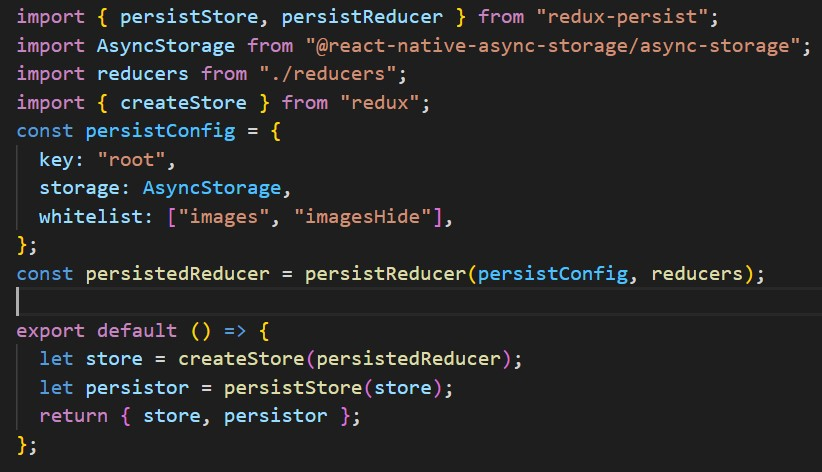
\includegraphics[width=10cm, height=7cm]{images/persistStore.jpg}
    \caption[differenzeiteot]{Creazione dello store persistente}
    \label{fig:persistStore}
\end{figure}

Come si pu\`o osservare nella fig 3.12, react-redux richiede che vengano indicati quali stati dello store debbano essere mantenuti in modo persistente e quali no; in questo applicativo solo gli state ``images" e ``imagesHide" vengono mantenuti in questo modo.
\`E necessario poi creare lo store utilizzando la configurazione persistConfig, fornita da react-redux.

Per completare la configurazione dello store persistente si deve ``avvolgere" il NavigationContainer, che a sua volta ``avvolge" l'intera applicazione, come mostrato nella fig 3.8.
\begin{figure}[h]
    \centering
    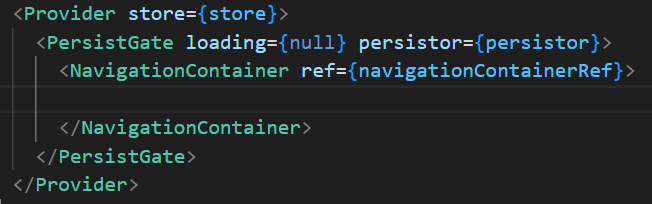
\includegraphics[width=10cm, height=4cm]{images/WrapNavigationConteiner.png}
    \caption[differenzeiteot]{Uso dello store persistente}
    \label{fig:usoStorePersistente}
\end{figure}

\section{Ripristinare le immagini occultate}
Una volta occultate, le immagini non vengono pi\`u visualizzate a meno che non sia l'utente a deciderlo. \`E stato realizzato un pulsante, chiamato ``Photos", che permette di ripristinare le immagini nascoste.

Nella schermata principale si hanno diversi pulsanti con uno stile simile, tra cui ``Photos": ho deciso quindi di realizzare un ``Custom component" in modo da poterlo riutilizzare per tutti i pulsanti.
Come si pu\`o osservare nella fig 3.14, a FilterButtonComponent {}(il ``Custom component") vengono passate cinque prop: tre per configurarne lo stile e due per configurarne il funzionamento.

Ogni volta che il pulsante Photos viene premuto, il suo colore cambia da azzurro a grigio e viceversa: questo avviene grazie alla prop ``setColor". 
Il cambio di colore indica una precisa azione del filtro:
\begin{itemize}
    \item Blu: vengono visualizzate anche le immagini nascoste. L'array ``images" contiene sia le foto da visualizzare che quelle nascoste, e vengono visualizzate solo quelle che possiedono la propriet\`a ``hide"= false; affinch\`e tutte le immagini vengano mostrate si deve settare la propriet\`a ``hide" 
          di ogni oggetto all'interno dell'array al valore ``false". Per poter aggiornare la FlatList \`e richiesto l'aggiornamento dello stato ``images" all'interno dello store.
    \item Grigio: vengono visualizzate solo le immagini che non sono state nascoste in precedenza.
        Per ritornare alla condizione in cui solo le immagini non occultate vengono visualizzate, viene invocata la funzione dontShowImagesHide(); questa va a ripristinare l'array ``images", andando a settare correttamente la propriet\`a ``hide" di ogni oggetto all'interno di esso.
        Per poter aggiornare la FlatList \`e richiesto l'aggiornamento dello stato ``images" all'interno dello store.
\end{itemize}

\begin{figure}[h]
    \centering
    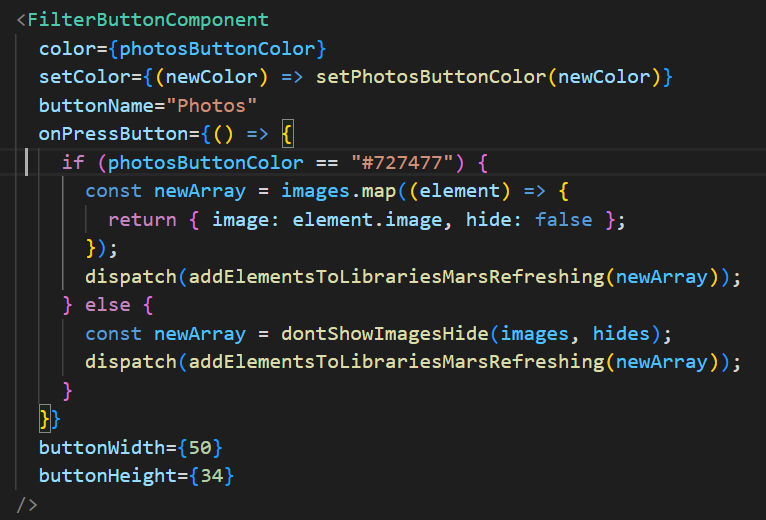
\includegraphics[width=11cm, height=8cm]{images/photoButton.png}
    \caption[differenzeiteot]{Filtro Photos}
    \label{fig:photoButton}
\end{figure}
\section{Procedura di Sign In e Sign Up}
Ogni utente prima di poter accedere all'applicazione deve disporre di un JWT (JSON Web Token); per poterlo ottenere \`e necessario fornire
e-mail e password nella schermata di login o di registrazione, a seconda che le credenziali siano gi\`a registrate nel database o meno.
Sia la procedura di \textit{sign in}  che quella di \textit{sign up} richiedono che venga contattato il server locale. In particolare, nella prima procedura viene 
contattata la route localhost3000/signin, mentre nella seconda viene contattata la route localhost3000/signup.
\begin{figure}[h]
    \centering
    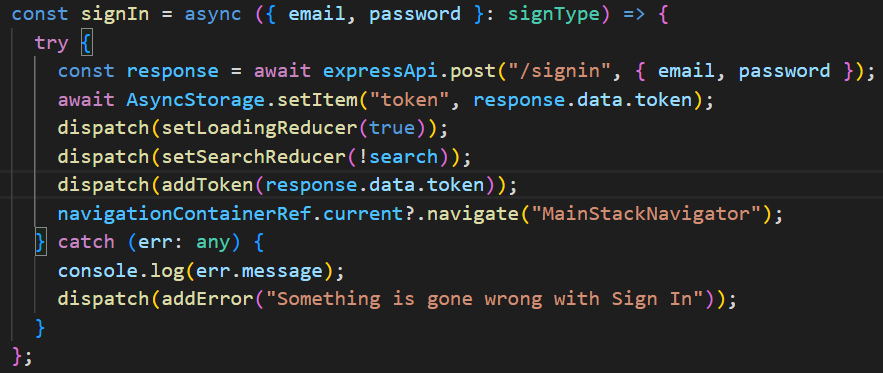
\includegraphics[width=10cm, height=5cm]{images/signInApplication.png}
    \caption[differenzeiteot]{Funzione di sign in}
    \label{fig:sign in}
\end{figure}

Come si pu\`o notare nella fig 3.15 l'utente invia un oggetto contenente la propria e-mail e password utilizzato il metodo post della libreria Axios;
il quale invier\`a l'oggetto in formato JSON.

Se la procedura di \textit{sign in} va andare a buon fine, il server risponde con il JWT dell'utente, il quale viene salvato all'interno dell'``asyncStorage"; cos\`i facendo quando l'utente riapre
l'applicazione non deve nuovamente inserire le proprie credenziali, ma viene automaticamente loggato all'interno dell'applicazione.\\
Se invece la procedura di \textit{sign in} non va a buon fine, viene mostrato un errore all'utente in modo che capisca che le proprie credenziali non sono corrette.

La procedura di \textit{sign up} \`e identica tranne per la route che l'applicazione contatta.

Vediamo ora nel dettaglio la route di \textit{sign in} e \textit{sign up} all'interno del server.
\subsection*{Sign Up}
Come si pu\`o vedere nella fig 3.16, la prima operazione svolta dalla route di \textit{sign up} consiste nell'andare ad estrarre le credenziali
fornite dall'utente; una volta ottenute viene creato e poi salvato un nuovo ``user" all'interno del database tramite il metodo ``save".

Se il salvataggio avviene correttamente, si genera un JWB che viene inserito nel body della risposta inviata dal server all'applicazione.
\begin{figure}[h]
    \centering
    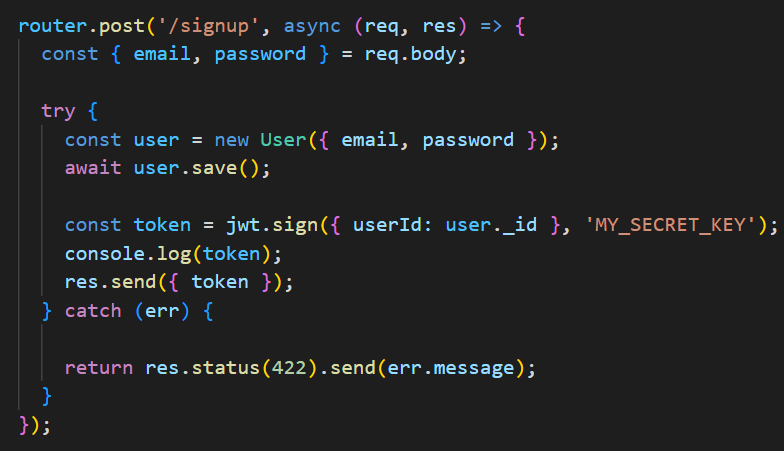
\includegraphics[width=10cm, height=6cm]{images/signUpServer.png}
    \caption[differenzeiteot]{Route di sign up}
    \label{fig:sign up}
\end{figure}

Prima di effettuare il salvataggio dell'utente nel database viene eseguita una operazione di pre-saving come mostrato nella fig 3.17. In questa operazione viene cifrata la password fornita dall'utente.
Per eseguire la cifratura vengono usati due metodi della libreria bcrypt; ossia genSalt e hash: in particolare, il secondo permette di eseguire l'hash
della password. Quest'ultima viene poi sostituita a quella inserita dall'utente in modo che venga inserita nel database.

\begin{figure}[h]
    \centering
    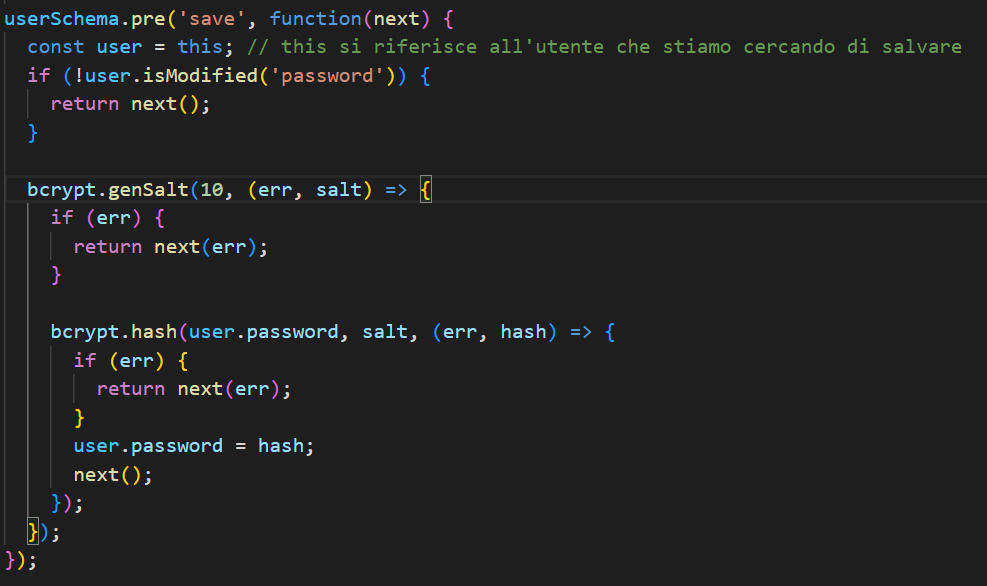
\includegraphics[width=9cm, height=6cm]{images/preSaveFunction.png}
    \caption[differenzeiteot]{Funzione di pre-saving}
    \label{fig:pre-saving}
\end{figure}


\subsection*{Sign In}

\begin{figure}[H]
   \centering
    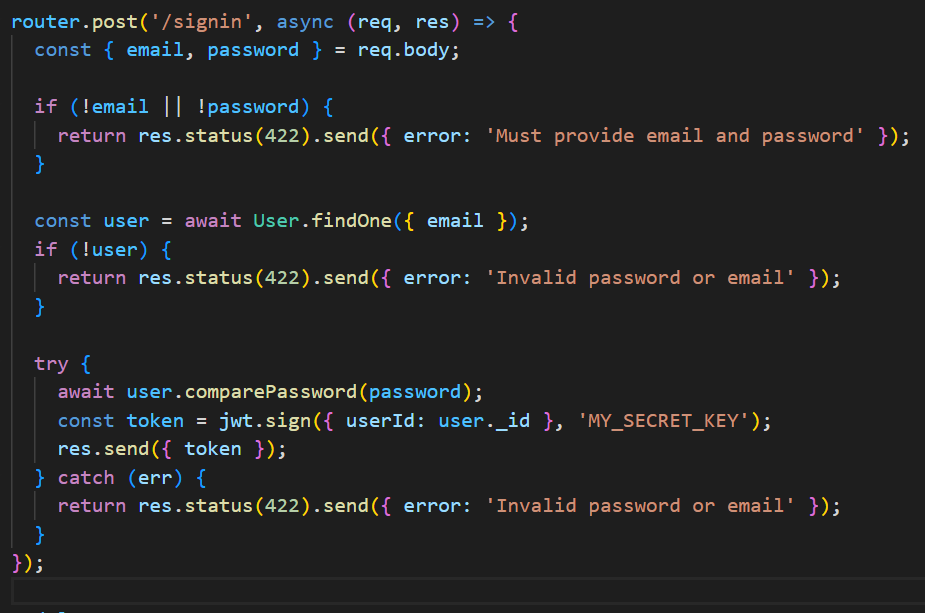
\includegraphics[width=9cm, height=6cm]{images/signinServer.png}
    \caption[differenzeiteot]{Route di sign in}
    \label{fig:Route sign in}
\end{figure}

Come si pu\`o vedere nella fig 3.18, per prima cosa si accede alle credenziali inviate dall'utente e si controlla che siano state fornite sia un'email che una password. In seguito, attraverso l'email fornita, viene recuperata la password cifrata presente
nel database e tramite la funzione comparePassword() si confrontano le due password. Questa funzione fa uso dl metodo compare del modulo bcrypt per andare a verificare che la password fornita dall'utente e quella cifrata presente sul database siano uguali.
 Se la verifica da esito positivo, viene generato un JWT tramite il metodo sign del modulo ``jsonwebtoken". il token generato viene poi inserito nel body della riposta per l'utente.
